\chapter{Conceptos Básicos}
\label{chap2}
\ifpdf
  \graphicspath{{Chapter2/Chapter2Figs/}}
\else
  \graphicspath{{Chapter2/Chapter2Figs/}}\fi

\markboth{\hfill \thechapter. Conceptos Básicos}{\hfill \thechapter. Conceptos Básicos}

\section{Imagen Digital}

% imagen gral
Una Imagen es una representación visual de un objeto real o imaginario que describe su apreciación visual en un momento dado. Puede ser un dibujo, una fotografía o una imagen digital \cite{russ2010}.

% definición matemática
Una imagen puede ser definida como una función de dos dimensiones, $F(i,j)$, donde $(i,j)$ son coordenadas espaciales, y el valor de $F(i,j)$ en cualquier par de coordenadas $(i,j)$ es llamado intensidad o nivel de gris  de la imagen en ese punto. Cuando los valores de $i$ y $j$ son cantidades discretas y finitas, llamamos a la imagen, \textbf{Imagen digital} $f(i,j)$.

\begin{figure}[H]\centering
    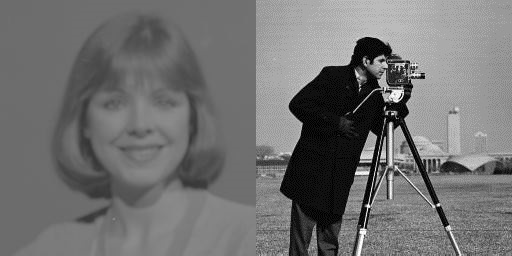
\includegraphics[width=0.7\textwidth]{ej_img_digitales.jpg}
    \caption{Ejemplos de imágenes digitales en escala de grises.}
    \label{fg:img_digital}
\end{figure}

% imagen digital
Una \textbf{imagen digital} es una imagen $F(i,j)$ que se ha discretizado (proceso de digitalización) tanto en coordenadas espaciales como en brillo, por tanto, se lo puede considerar como una matriz de dimensiones M x N, donde $(i,j)$ identifica un punto en la imagen y el valor correspondiente del elemento de la matriz indica el nivel de gris en ese punto. Los elementos de una distribución digital de este tipo se denominan elementos de la imagen o pixeles \textbf{$p$}. En la Ecuación \ref{representacion_imagen_digital} se observa la representación de una imagen como matriz.

\begin{equation}
F(i,j) = 
\begin{pmatrix} 
f({0,0}) & f({0,1}) & \ldots & f({0,N-1}) \\
f({1,0}) & f({1,1}) & \ldots & f({1,N-1}) \\
f({2,0}) & f({2,1}) & \ldots & f({2,N-1}) \\ 
\ldots & \ldots & \ldots &  \ldots \\
f({M-1,0}) & f({M-1,1}) & \ldots & f({M-1,N-1})
\end{pmatrix}  
\label{representacion_imagen_digital}
\end{equation}

% como se obtiene una imagen digital?
El proceso de digitalización de una imagen consiste en dividir la imagen en pequeñas regiones llamadas elementos de imagen o pixeles \textbf{$p$}, medir el nivel de gris de la imagen para cada píxel (intensidad), cuantificar esa medición continua para producir un valor entero y luego generar una salida.

El píxel \textbf{$p$} (del inglés picture element) es el elemento más pequeño que forma la imagen, es interpretado generalmente como una entidad cuadrada o rectangular. En la Figura \ref{imagen_pixeles} se muestra la representación de una imagen de 8x8 pixeles y la matriz correspondiente a la imagen con el valor de la intensidad de cada píxel.

\begin{figure}[H]
    \begin{center}
        \subfigure[][\label{fig:label:1} Imagen de 8x8 pixeles]{
\includegraphics[width=7cm]{imagen8x8_pixeles.png}}
        \subfigure[][\label{fig:label:2} Matriz de la imagen de 8x8 pixeles]{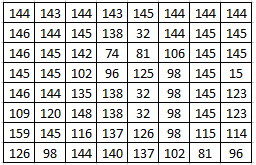
\includegraphics[width=7cm]{matriz8x8_pixeles.png}}
    \end{center}
    \caption{Representación de una imagen y sus elementos de imagen o pixeles}
    \label{imagen_pixeles}
\end{figure}

Las imágenes en escala de gris utilizan niveles de gris donde cada nivel equivale a una graduación de gris comprendido entre el negro y el blanco \cite{russ2010}. La cantidad de niveles de gris de la escala depende de la cantidad de bits tomados para representar un nivel de gris. Por ejemplo, si se utilizan 8 bits, se puede representar 256 niveles de gris distintos que van del 0 (negro) al 255 (blanco).
% Un bit es la unidad de medida mínima de información empleada en el campo de la computación y la información digital \cite{oceano2000}. La escala más utilizada es la de 8 bits con lo que se puede representar 256 niveles de gris distintos que van del 0 (negro) al 255 (blanco).

En la Figura \ref{niveles_gris}, se muestran ejemplos de niveles de gris en base a la cantidad de bits tomados. Con 1 bit, se puede representar 2 niveles, el 0 (negro) y el 1 (blanco), con lo que solo se pueden formar imágenes monocromáticas. Con 2, 3, 4, 5, 6 y 7 bits se pueden representar 4, 8, 16, 32, 64 y 128 niveles de gris respectivamente.\break

\begin{figure}[H]
  \begin{center}
    \leavevmode
    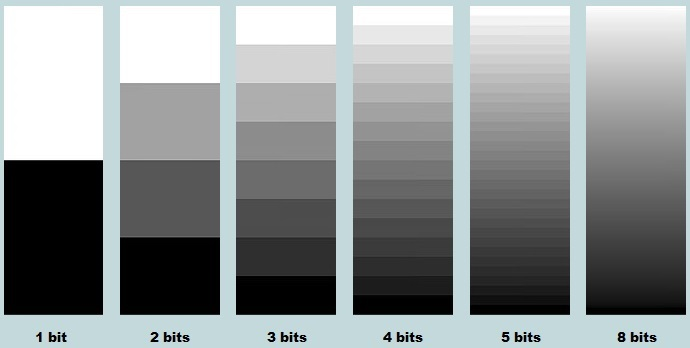
\includegraphics[width=15cm] {niveles_gris.png}
    \caption{Niveles de gris.}
    \label{niveles_gris}
  \end{center}
\end{figure}

En la Figura \ref{imagen_pixelada} se muestra una imagen en escala de gris y una sección de la imagen en el que se observan sus pixeles individuales (imagen pixelada).

\begin{figure}[H]
  \begin{center}
    \leavevmode
    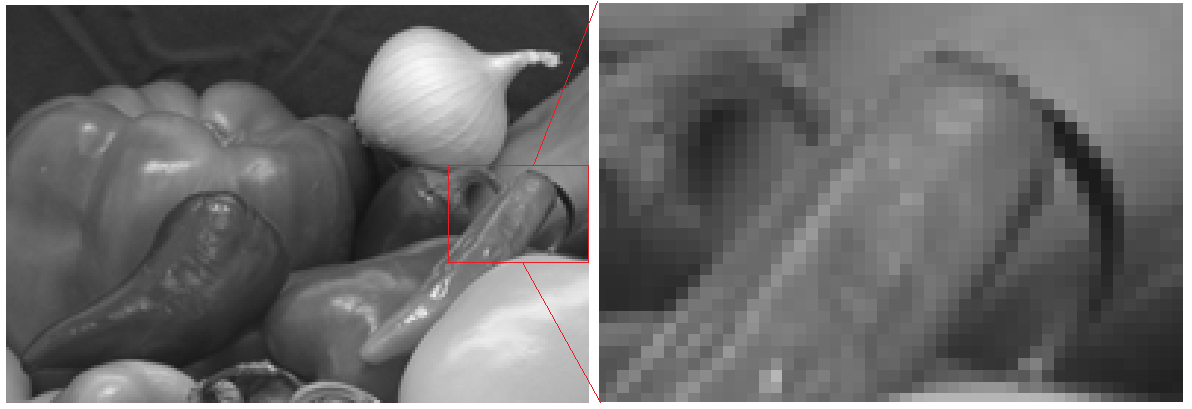
\includegraphics[width=14cm] {imagen_pixelada.png}
    \caption{Pixeles de una imagen digital en escala de grises.}
    \label{imagen_pixelada}
  \end{center}
\end{figure}


\section{Mejora de imagen}

La \textit {Mejora de Imagen} consiste en un conjunto de técnicas que se aplican a las imágenes con el objetivo de mejorar su calidad, ya sea en contraste, ruido, distorsiones, luminosidad, falta de nitidez; destacar algún aspecto de la información contenida en la misma; procesar y/o analizar una imagen, de tal modo que la resultante sea más adecuada que la imagen original, para cierta aplicación específica \cite{gonzales1996procesamiento}.

Es importante destacar que, al utilizar algoritmos de mejora de la imagen, normalmente se consideran los siguientes aspectos:

\begin{itemize}
  \item No se añade información nueva que no esté presente en la imagen. Tan solo se resalta la información existente, para que pueda ser apreciada de mejor manera por el ojo humano.
  \item La valoración de los resultados es subjetiva, debido a que no existe un criterio para saber que tanto se mejoró la imagen original, por lo regular se emplean varias pruebas sobre la imagen hasta obtener los resultados más adecuados.
\end{itemize}

La Mejora de Imagen consiste en la transformación de las intensidades para el realzado de imágenes, conduce a un cambio de brillo y/o contraste de la imagen. Las técnicas consisten en operaciones directamente sobre un píxel sin tomar en cuenta a los pixeles vecinos, que sirve para mejorar condiciones de bajo contraste, baja luminosidad o demasiada obscuridad; y operaciones sobre un píxel tomando en cuenta a los pixeles que lo rodean, lo cual ayuda a eliminar ruido o para el mejoramiento de la nitidez.

La Mejora de Imagen es una de las áreas más simples y más atractivas del procesamiento digital de imágenes. El objetivo de las técnicas de mejora es resaltar los detalles que se ocultan, o simplemente resaltar ciertas características de interés en una imagen. Es importante tener en cuenta que la mejora es un área subjetiva en el procesamiento de imágenes, ya que el resultado obtenido es evaluado por un ser humano; es decir, el encargado de determinar en cuánto una técnica ha mejorado cierto aspecto de una imagen es un experto en la materia \cite{handbook2000}.

\section{Contraste}

El \textit{Contraste} se define como la diferencia relativa en la intensidad entre un punto de una imagen y sus alrededores. Eso se traduce en la diferencia entre la luminosidad de los diferentes objetos de una imagen que los hace distinguibles a los unos de los otros \cite{russ2010}.

La lumunosidad o brillo es la cantidad de luz emitida o reflejada por un objeto.  Y en un color sería su claridad u oscuridad.

El contraste separa las características más esenciales de un elemento o puede realizarse la evaluación de similitud de las cosas para determinar la visibilidad de puntos con determinados tipos de luz. Una imagen con mucho contraste muestra una variación más acusada en su escala de grises.

En la Figura \ref{contraste} todos los cuadrados internos tienen la misma intensidad, pero aparecen progresivamente más oscuros a medida que el fondo se hace más claro.

% \hfill \begin{figure}[!htbp]
\begin{figure}[H]
  \begin{center}
    \leavevmode
    
\includegraphics[height=4.7cm]{ej_contraste.png}
    \caption{Ejemplo de contraste.}
    \label{contraste}
  \end{center}
\end{figure}

Cuanto mayor sea el contraste, más se incrementa el cambio de luminosidad entre las zonas oscuras o claras de una imagen, simulando, un mejor enfoque y claridad en la imagen.


\section{Mejora de Contraste}

La \textit{Mejora de Contraste} es una técnica cuyo efecto es mejorar o incrementar la visibilidad de los detalles de una imagen, comprende un conjunto de transformaciones sobre los tonos de gris de los pixeles de la imagen para mejorar la apariencia de la misma y hacerla más apta para la visión humana \cite{kwok2006}.

En la Figura \ref{mejora_contraste}, se muestran una imagen con poco contraste y la imagen resultante al mejorar el contraste de la misma imagen.

\begin{figure}[H]
    \captionsetup[figure]{labelformat=empty}
    \centering
        \subfigure[][]{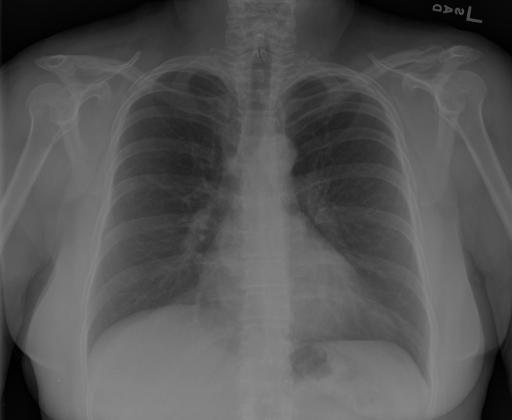
\includegraphics[width=6cm]{imagen12.png}}
        \subfigure[][]{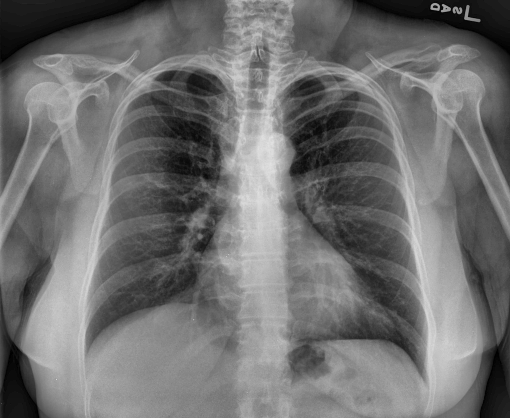
\includegraphics[width=6cm]{imagen12_clahe.png}}
    \caption{Imagen Original (a), Imagen mejorada (b)}
    \label{mejora_contraste}
\end{figure}

La idea en este tipo de transformación es modificar los valores de los pixeles de manera que se produzca un aumento en el rango dinámico de los valores de niveles de gris de la imagen, modificar los niveles de gris oscuros por unos más claros y viceversa y así aumentar la diferencia de intensidad entre los pixeles \cite{kwok2006}.

La Mejora del Contraste permite distinguir objetos en la imagen que no son distinguibles cuando se produce pérdida de contraste debido principalmente a la iluminación deficiente \cite{kwok2006}.

Al modificar los valores de los pixeles se altera la estructura de la imagen y esto puede causar problemas como la distorsión o degradación de la imagen, que se atribuye a una mala reasignación de los niveles de gris. Esto ocasiona la pérdida de información y de visualización correcta de algunos detalles de la imagen \cite{kwok2013}. Además, existen los problemas de amplificación de ruido y artefactos, que consisten en el aumento en la diferencia de intensidad en el brillo entre dos o más pixeles entre sí que se hace más visible y no es parte de la escena capturada en la imagen, que puede ser causada por los dispositivos de captura de imágenes. Los artefactos son objetos extraños que no existen en la imagen original y que pueden surgir luego de una modificación inadecuada de la imagen o como una amplificación grave de ruido \cite{kwok2013}.

Para resolver estos problemas, los algoritmos de mejora de contraste se utilizan en conjunto con métricas de evaluación que determinan la calidad del resultado. La \textbf{Métrica de evaluación} es una medida de semejanza entre la imagen original y la distorsionada, que mide la degradación de la imagen, la perdida de información y la adición de ruidos provocados por una mala modificación de los pixeles.
La Mejora del Contraste se puede clasificar en dos, el enfoque de \textit{mejora global} y el enfoque de \textit{mejora local} \cite{morebrizuela2014}. Para la selección del enfoque, se debe estudiar qué tipo de imágenes serán procesadas o qué tipo de interés está motivando la mejora de contraste.

\subsection{Mejora de Contraste Global}

En el enfoque global el valor de salida para un píxel específico depende de los valores de todos los puntos de la imagen de entrada, transforman los datos originales usando las estadísticas calculadas para toda la imagen. Opera sobre toda la imagen a la vez.

Con el enfoque global no siempre se consigue resaltar todos los detalles de la imagen. Aplican una función de transformación cuya forma está basada en la distribución de los niveles de intensidad de una imagen completa. Aunque este método puede mejorar el contraste total y el rango dinámico de una imagen, existen casos en donde se desea la mejora de detalles sobre regiones pequeñas. La solución en este caso es derivar una transformación basada sobre la distribución de intensidades en la vecindad local de cada píxel en la imagen \cite{procesamientoimagen}.

\subsection{Mejora de Contraste Local}

Si se usa sólo información global no se alcanza una buena mejora de contraste, debido a que las técnicas globales causan un efecto de saturación de intensidades \cite{yu2004fast}. 

% En imágenes, la saturación es un tipo de distorsión donde la imagen grabada se limita a algún valor máximo, lo que interfiere con la medición de las regiones brillantes de la escena.
% Los pixeles saturados contienen menos información sobre la escena que otros pixeles.

En la Figura \ref{saturacion_intensidad} se muestra un ejemplo del cambio de las intensidades de los tonos o color (saturación de intensidades).

% Coloquialmente, un píxel por encima de 255 o por debajo de 0 se dice que está saturado.
% La saturación supone una pérdida de información

\begin{figure}[H]
    \captionsetup[figure]{labelformat=empty}
    \centering
        
\includegraphics[width=10cm]{saturacion_intensidad.jpg}    
        \caption{Ejemplo de Saturación de Intensidades}
    \label{saturacion_intensidad}
\end{figure}
 
En el enfoque local, el valor de salida para un píxel específico depende de los valores de entrada de sus vecinos más próximos y del propio píxel en la imagen original.

La mejora se realiza dividiendo la imagen por bloques (vecindades) y se aplica la función de transformación a cada bloque independientemente. De esta forma, cada bloque es tratado como si fuera una imagen aparte y se mejora el contraste en cada una de ellas independientemente. Finalmente se unen las partes mejoradas a través de alguna técnica de unión. Esta técnica permite revelar estructuras finas de la imagen en algunas situaciones.

En la Figura \ref{imagenes_bloques} se muestra la imagen dividida en bloques y la imagen resultante al mejorar cada bloque independientemente.

\begin{figure}[H]
    \centering
        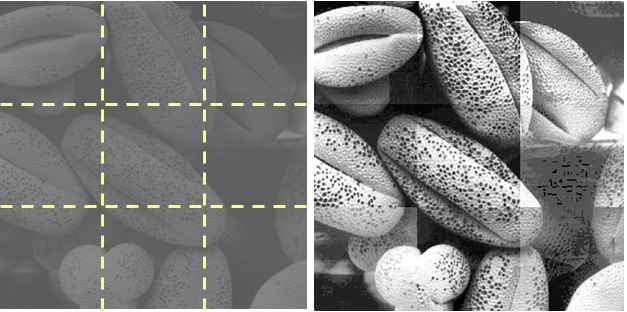
\includegraphics[width=10cm]{ej_imagen_bloques.png}    
        \caption{Imagen dividida y mejorada por bloques.}
    \label{imagenes_bloques}
\end{figure}

De esta forma la técnica de mejora local puede mejorar el contraste de manera más eficaz.

%en las técnicas locales de mejora, el costo computacional es muy alto debido a sus sub-bloques que se superponen completamente y causa sobrerealce en algunas partes de la imagen.

% El hecho de considerar los pixeles de una vecindad, hace que las técnicas de procesamiento basadas en una región tengan un mayor costo de cálculo numérico que las técnicas basadas en un solo punto. Este costo dependerá del tamaño de la vecindad a considerar, así como del tipo de representación numérica utilizada. Sin embargo, para la mayoría de las aplicaciones y con las computadoras disponibles actualmente, se pueden obtener muy buenos resultados en términos de tiempo de cálculo, al procesar imágenes de un tamaño mediano (256 x 256 ó 512 x 512).

\section{Histograma de Niveles de Gris}

% definicion matemática
El $Histograma$ de una imagen se define como la representación gráfica de la distribución de frecuencias de la imagen, en este caso, la cantidad de pixeles que posee cada nivel de intensidad considerada en el rango \cite{SMG11}.

El histograma $\mathcal{H}$ asociado a la imagen que describe la frecuencia de los valores de intensidades $k$ que aparecen en la misma, se puede expresar como sigue \cite{kwok2013}:

\begin{equation}
    \label{ecuacion_histograma}
    \mathcal H_{k} = \lbrace n_k \rbrace \qquad %siendo\qquad Z=\sum_{k=1}^{L}n_{k}
\end{equation}

Donde:
\begin{itemize} 
    \item $\mathcal{H}$ es el histograma;
    \item $k = [0, L-1] \quad \forall \quad k \in \mathbb{N}$;
    \item $L-1$ es el máximo nivel de gris disponible. 
    \item $n_k$ es el número de ocurrencia de la intensidad $k$ en la imagen;
  %  \item $Z$ es la cantidad total de pixeles de la imagen.
\end{itemize}

La forma del histograma permite evidenciar ciertas particularidades de la imagen, como lo son el tipo de fondo, el contraste y en general si los valores de los niveles de gris están homogéneamente distribuidos o no. El histograma podría ser alterado para producir cambios en la imagen. En la Figura \ref{cameraman-histograma} se observa el histograma de una imagen.
%imagen oscura: el rango de niveles concentrados hacia la izquierda
%imagen clara: el rango de niveles concentrados hacia la derecha

\begin{figure}[H]
    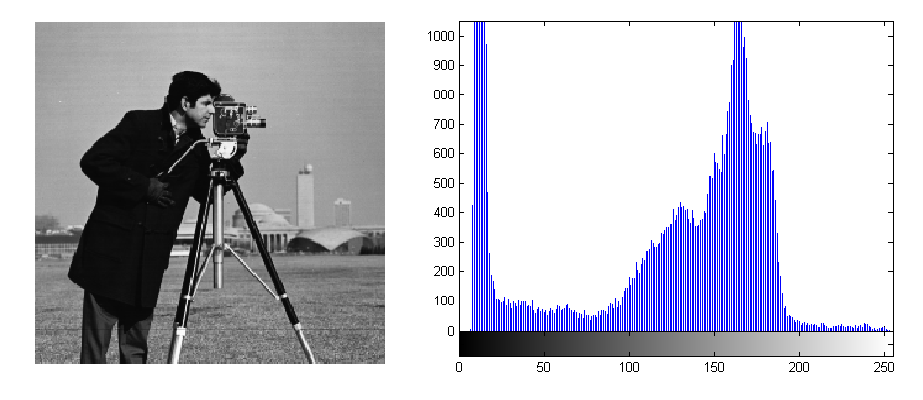
\includegraphics[width=14cm]{cameraman-histograma.png}
    \caption{Imagen Cameraman y su respectivo histograma.}
    \label{cameraman-histograma}
\end{figure}

En la Ecuación \ref{imagen_4x4} se representa una imagen como una matriz de dimensiones 4x4 pixeles, en la Figura \ref{representacion_histograma} se muestra la representación del histograma de la matriz 4x4, en el cual se puede observar sus intensidades $k$ y las ocurrencias $n_k$ de cada valor de $k$. Por ejemplo, para la intensidad $k=2$, se observa que el número de ocurrencias en la matriz es $n_k=4$.

\begin{equation}
f(i,j) = 
\begin{pmatrix} 0 & 1 & 2 & 3 
\\4 & 5 & 0 & 2 
\\3 & 4 & 5 & 2 
\\4 & 5 & 2 & 4
\end{pmatrix} 
\label{imagen_4x4}
\end{equation}

\begin{figure}[H]
    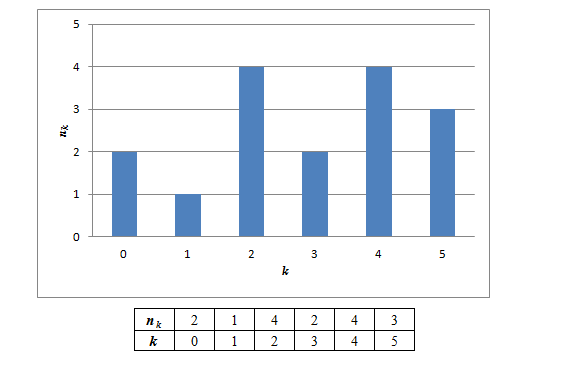
\includegraphics[width=14cm] {representacion_histograma.png}
    \caption{Representación del histograma correspondiente a la imagen representada por la matriz en la ecuación \ref{imagen_4x4}}
    \label{representacion_histograma}
\end{figure}

Las técnicas de modificación del histograma de una imagen son útiles para aumentar el contraste de las imágenes con histogramas muy concentrados, ya sean imágenes oscuras como claras. 

Cuando el rango de niveles de gris que toma la imagen se encuentra concentrado en una zona del intervalo, la imagen posee poco contraste. Para aumentar el contraste, podemos expandir el Histograma o bien realizar una ecualización sobre el mismo. La ecualización consiste en la distribución uniforme de sus intensidades sobre toda la escala de grises, sección \ref{sec:ecualizacion_histograma}.

Muchas imágenes tienen histogramas muy dispersos y concentrados. Por ello, transformarlos en un histograma más uniforme causa una distorsión o una sobre mejora de contraste que afectan considerablemente a la correcta visualización de la misma \cite{PTS+13}.

En la Figura \ref{imagen25_hist_ori} se muestra una imagen con su histograma más al lado izquierdo, esto nos indica que se trata de una imagen oscura.

\begin{figure}[H]
    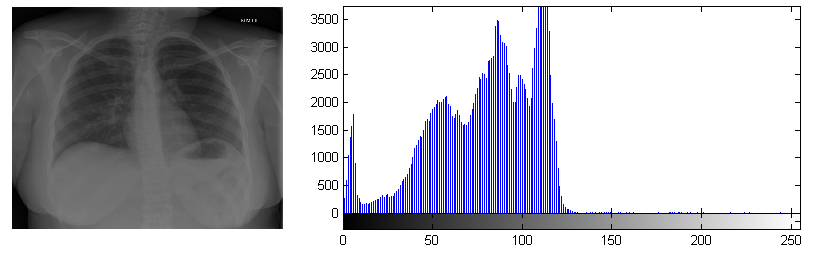
\includegraphics[width=15cm]{imagen25_Hist_Ori.png}
    \caption{Imagen original y su respectivo histograma.}
    \label{imagen25_hist_ori}
\end{figure}

En la Figura \ref{imagen25_hist_ecua} se muestra el resultado de realizar una ecualización al histograma de la imagen, se obtiene un histograma más disperso, con picos en el lado derecho del histograma, lo que nos da una imagen con zonas más claras.

\begin{figure}[H]
    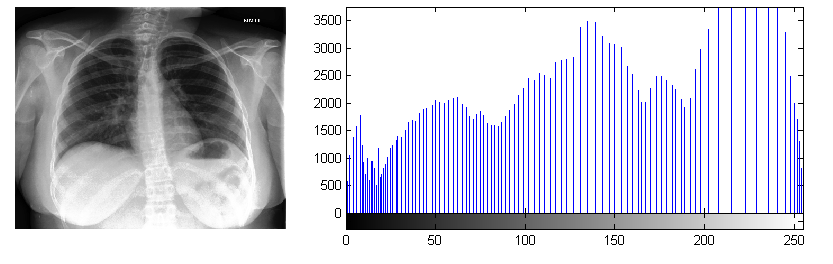
\includegraphics[width=15cm] {imagen25_Hist_Ecua.png}
    \caption{Imagen ecualizada y su respectivo histograma.}
    \label{imagen25_hist_ecua}
\end{figure}


\subsection{Ecualización Clásica del Histograma}
\label{sec:ecualizacion_histograma}

La \textit{Ecualización del Histograma} ($HE$ por sus siglas en inglés Histogram Equalization), consiste en tratar de transformar el histograma de la imagen en un histograma lo más uniforme posible. Un histograma normalizado o uniforme es aquél en el que la variable representada ha sido escalada para ajustarse a un rango entre 0 y 1. Es decir, que exista el mismo número de pixeles para cada nivel de gris del histograma \cite{byong2013}.

La técnica consiste en la manipulación del histograma para mejorar el contraste en las áreas muy claras o muy oscuras de una imagen, así como también expandir los niveles de gris a lo largo de todo el intervalo. Se consigue utilizando como función de transformación la distribución acumulativa de la intensidad. Esta técnica está basada en la teoría de probabilidades, tratando al histograma como una distribución de probabilidad de los niveles de gris.

El resultado de la ecualización maximiza el contraste de una imagen sin perder información de tipo estructural.

En la ecuación \ref{representacion_imagen_6x6} se representa a una imagen como matriz de 6x6 pixeles; donde se define:
\begin{itemize}
    \item Total de pixeles en la imagen: $Z=M \times N=36$.
    \item Niveles de gris: $L=16$; porque es la menor potencia de 2 capaz de capturar todos los 14 valores de intensidades expresados en la matriz.
\end{itemize}

\begin{equation}
f(i,j) = 
 \begin{pmatrix} 
 0 & 9 & 10 & 12 & 9 & 0 \\
 10 & 0 & 11 & 10 & 11 & 0 \\
 9 & 11 & 9 & 11 & 10 & 12 \\
 10 & 12 & 10 & 0 & 12 & 9 \\
9 & 9 & 10 & 12 & 12 & 10 \\
12 & 12 & 10 & 13 & 13 & 10 \\
\end{pmatrix}
\label{representacion_imagen_6x6}
\end{equation}

A partir de la representación de la imagen como matriz, en la ecuación \ref{representacion_imagen_6x6}, se puede aplicar la técnica $HE$, obteniendo:
\begin{enumerate}
  \item \textit{Frecuencia absoluta o $PMF$ (por sus siglas en inglés Probability Mass Function)}: se cuenta el número de ocurrencias para cada nivel de gris ($k$).
  
    \begin{figure}[H]
    \centering
        \begin{tabular} {| c | c | c | c | c | c | c | c | c |c | c | c | c | c | c | c | c |} \hline
                \textbf{k} & 0 & 1 & 2 & 3 & 4 & 5 & 6 & 7 & 8 & 9 & 10 & 11 & 12 & 13 & 14 & 15 \\ \hline
                \textbf{PMF} & 5 & 0 & 0 & 0 & 0 & 0 & 0 & 0 & 0 & 7 & 10 & 4 & 8 & 2 & 0 & 0 \\ \hline
        \end{tabular}
        \caption{Ecualización del histograma - Cálculo de la frecuencia absoluta.}
        \label{tabla_frecuencia_absoluta}
    \end{figure}
    
    \begin{figure}[H]
    \centering
        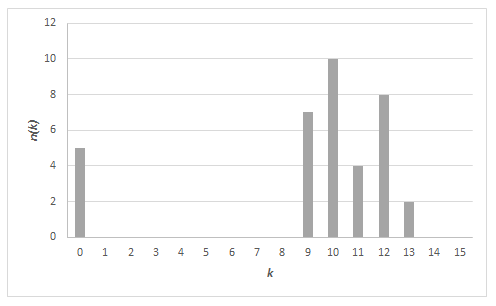
\includegraphics[width=14cm] {histograma_matriz_6x6.png}
        \caption{Representación del histograma correspondiente a la imagen representada por la matriz 6x6.}
        \label{representacion_histograma_6x6}
    \end{figure}

 \item \textit{Función de Distribución Acumulativa $FDA$}: se acumulan los valores de la frecuencia absoluta. $FDA$ nos da la suma acumulativa de los valores calculados en el paso 1 y se puede expresar como sigue:
    \begin{equation} \label{fda}
        FDA_{f(i,j)}(k)=\sum_{k=0}^{L-1} \frac{n_k}{Z}
    \end{equation}
    
    donde:
    \begin{itemize}
        \item $f(i,j)$ es la imagen de entrada.
        \item $L-1$ es el nivel máximo de gris de la imagen.
        \item $\frac{n_k} {Z}$ es la cantidad de pixeles normalizada del $k$-ésimo nivel de gris.
    \end{itemize} \break
    
    En la Ecuación \ref{fda} se muestra el cálculo de $FDA$ para cada píxel de la imagen representada por la matriz 6x6. 
    
    \begin{align}
        \begin{split}
            FDA(0) ={}& \frac{5}{36}\\
            \ldots\\
            FDA(8) ={}& \frac{5}{36}\\
            FDA(9) ={}& \frac{12}{36}\\ 
            \ldots\\
            FDA(12) ={}& \frac{34}{36}\\
            \ldots\\
            FDA(15) ={}& \frac{36}{36}
        \end{split}
        \label{fda_6x6}
    \end{align}
    
    \item Se multiplican los valores normalizados por el máximo valor de nivel de gris y se redondean. El valor calculado por $FDA$ se multiplica por el máximo nivel de gris, para encontrar las nuevas intensidades de pixeles. \\
    \begin{equation} \label{ecualizado}
        Ecualizado(k)= \left \lceil (L-1) * FDA(k)) \right \rceil
    \end{equation}
    
    Siguiendo el mismo proceso práctico, tenemos:
    
     \begin{align}
        \begin{split}
    Ecualizado(0) ={}& \left \lceil 15 * \frac{5}{36} \right \rceil  = 2  \\
    \ldots\\
    Ecualizado(8) ={}& \left \lceil 15 * \frac{5}{36} \right \rceil  =  2  \\
    Ecualizado(9) ={}&  \left \lceil 15 * \frac{12}{36} \right \rceil  = 5  \\
    \ldots\\
    Ecualizado(12) ={}&  \left \lceil 15 * \frac{34}{36} \right \rceil  = 14  \\
    \ldots\\
    Ecualizado(15) ={}& \left \lceil 15 * \frac{36}{36} \right \rceil  = 15 \\
           \end{split}
    \end{align}

  \item Se modifican los valores de gris asignando los niveles de gris ecualizados; $k$ representa a los niveles de gris originales de la matriz, por otro lado, $k'$ representa los niveles de gris finales, es decir $k'$ = Ecualizado (k) ver ecuación \ref{ecualizado}.
  
    \begin{figure}[h]
    \centering
        \begin{tabular}{| c | c | c | c | c | c | c | c | c |c | c | c | c | c | c | c | c |} \hline
                \textbf{k}  & 0 & 1 & 2 & 3 & 4 & 5 & 6 & 7 & 8 & 9 & 10 & 11 & 12 & 13 & 14 & 15 \\ \hline
               \textbf{k'} & 2 & 2 & 2 & 2 & 2 & 2 & 2 & 2 & 2 & 5 & 9 & 11 & 14 & 15 & 15 & 15 \\ \hline
        \end{tabular}
        \caption{Ecualización del histograma - Niveles de gris ecualizados}
        \label{tabla_ecualizados}
    \end{figure}
    
   Finalmente, se muestran los resultados luego de aplicar la ecualización del histograma, en la ecuación \ref{imagen_6x6_ecualizado} se muestra cómo queda la nueva matriz que representa a la imagen de salida $f(x,y)$, en la Figura \ref{FDA_niveles_finales} se muestra el resultado del cálculo de la frecuencia absoluta para los valores de los nuevos pixeles; y en la Figura \ref{histograma_ecualizado_6x6} se muestra el histograma ecualizado.
    
    \hfill\begin{equation}
        f(i,j) = 
         \begin{pmatrix} 
         2 & 5 & 9 & 14 & 5 & 2 \\
         9 & 2 & 11 & 9 & 11 & 2 \\
         5 & 11 & 5 & 11 & 9 & 14 \\
         9 & 14 & 9 & 2 & 14 & 5 \\
        5 & 5 & 9 & 14 & 14 & 9 \\
        14 & 14 & 9 & 15 & 15 & 9 \\
        \end{pmatrix} 
        \label{imagen_6x6_ecualizado}
    \end{equation}
      
   \hfill\begin{figure}[h!]
   \centering
        \begin{tabular}{| c | c | c | c | c | c | c | c | c |c | c | c | c | c | c | c | c |} \hline
                \textbf{k'}  & 0 & 1 & 2 & 3 & 4 & 5 & 6 & 7 & 8 & 9 & 10 & 11 & 12 & 13 & 14 & 15 \\ \hline
                \textbf{PMF} & 0 & 0 & 5 & 0 & 0 & 7 & 0 & 0 & 0 & 10 & 0 & 4 & 0 & 0 & 8 & 2 \\ \hline
        \end{tabular}
        \caption{Ecualización del histograma - Cálculo de la frecuencia absoluta para los pixeles finales luego de la Ecualización del histograma.}
        \label{FDA_niveles_finales}
    \end{figure}
    
        \begin{figure}[H]
        \centering
        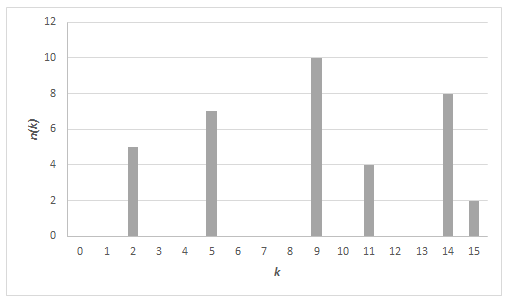
\includegraphics[width=14cm]{histograma_matriz_6x6_ecualizado.png}
        \caption{Representación del histograma ecualizado correspondiente a la imagen representada por la matriz en la ecuación \ref{imagen_6x6_ecualizado}}
        \label{histograma_ecualizado_6x6}
    \end{figure}
\end{enumerate}


$HE$ no está libre de inconvenientes. El estiramiento de contraste está limitado a los niveles de gris con mayor frecuencia. Esto causa una pérdida significativa de contraste para los niveles con menor frecuencia \cite{hashemi2009}. En esta situación, la ecualización del histograma reasigna los niveles de gris restringiendo el estiramiento de contraste hacia los niveles dominantes, causando una pérdida considerable al resto de los niveles de gris \cite{Shanmugavadivu2011}.

$HE$ es un proceso del enfoque de \textbf{mejora global}. El histograma se construye en base a todos los pixeles de la imagen y se procesa completamente. La desventaja de este proceso es que no considera la información local de cada píxel, de modo que puede existir bajo contraste en regiones pequeñas, también en ocasiones, esta técnica puede causar efectos no deseables y reducir la calidad de visualización, sufre de amplificación de ruido, sobre mejora de imagen, pérdida de detalles o distorsión, en las Figuras \ref{ampliacion_ruido}, \ref{sobremejora} y \ref{distorsion} se pueden observar ejemplos de estos efectos no deseables, causados por una mala redistribución de los pixeles a lo largo del histograma \cite{chulwoo2013,byong2013,PTS+13}.

\begin{figure}[H]
\centering
    \captionsetup[figure]{labelformat=empty}
        \subfigure[][]{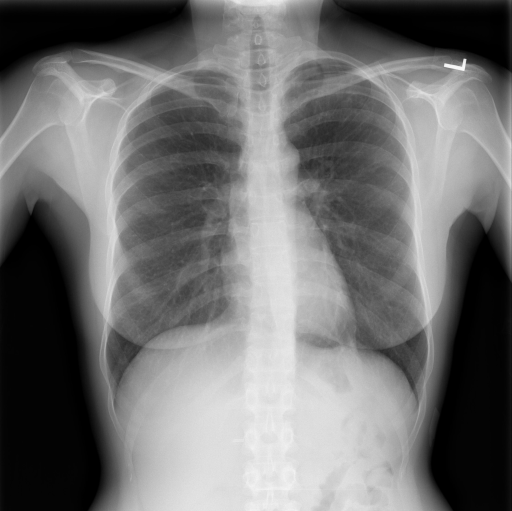
\includegraphics[width=5cm]{imagen10.png}}
        \subfigure[][]{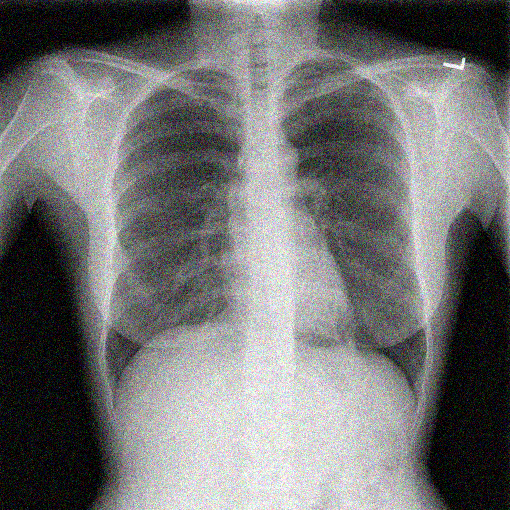
\includegraphics[width=5cm]{imagen10_ruido.png}}
    \caption{(a) Imagen Original. (b) Amplificación de ruido.}
    \label{ampliacion_ruido}
\end{figure}

\begin{figure}[H]
    \captionsetup[figure]{labelformat=empty}
    \centering
        \subfigure[][]{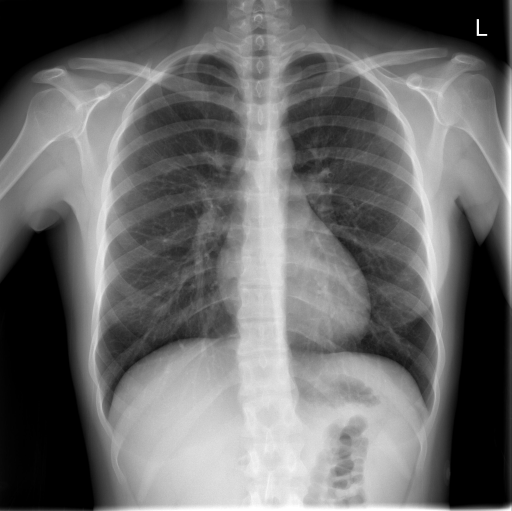
\includegraphics[width=5cm]{imagen4.png}}
        \subfigure[][]{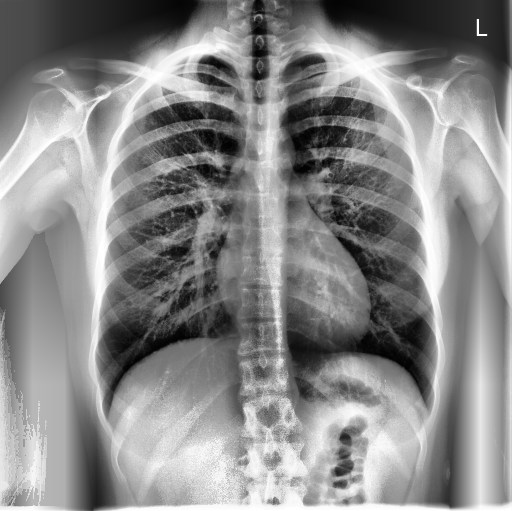
\includegraphics[width=5cm]{imagen4_sobremejora.png}}
    \caption{(a) Imagen Original. (b) Sobre mejora de imagen.}
    \label{sobremejora}
\end{figure}

\begin{figure}[H]
    \captionsetup[figure]{labelformat=empty}
    \centering
        \subfigure[][]{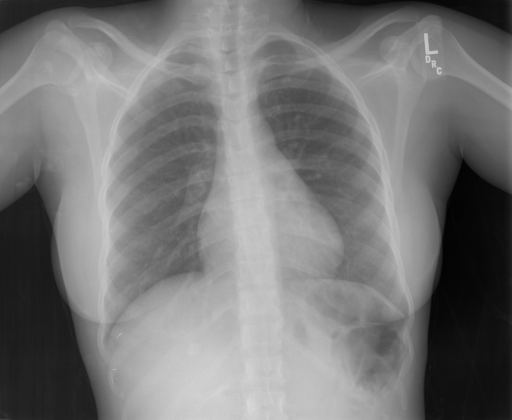
\includegraphics[width=5cm]{imagen2.png}}
        \subfigure[][]{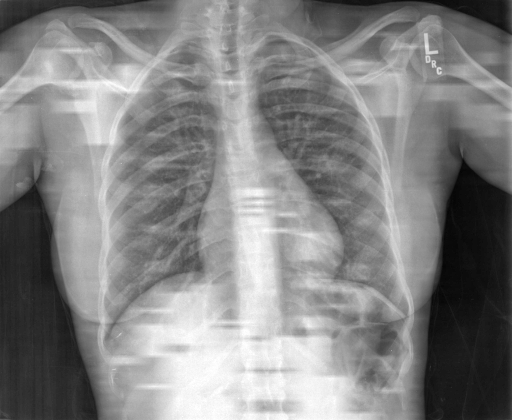
\includegraphics[width=5cm]{imagen2_distorsion.png}}
    \caption{(a) Imagen Original. (b) Perdida de detalles y distorsión.}
    \label{distorsion}
\end{figure}

Debido a estos efectos no deseados, se han desarrollado técnicas de división del histograma de la imagen, con lo que surge el concepto de ecualización local del histograma, basado en el enfoque de mejora local. 

\subsection{Ecualización Local del Histograma}

La \textit{Ecualización Local del Histograma} se realiza por bloques de la imagen en donde se ecualizan de forma independiente. Permite revelar estructuras finas de la imagen en algunas situaciones \cite{chulwoo2013}.

El procedimiento consiste en definir una vecindad, mover el centro de esta área píxel a píxel. En cada píxel, se calcula el histograma de la vecindad y se realiza la ecualización del histograma. Esta función de mapeo se aplica al píxel central de la vecindad. El píxel central se mueve a la siguiente posición y el esquema se repite.


\subsection{Adaptive Histogram Equalization (AHE)}

$AHE$ \cite{chulwoo2013}, (por sus siglas en inglés \textit{Adaptive Histogram Equalization}) procesa la imagen por subregiones (regiones rectangulares de la imagen), o {\it regiones contextuales}, con dimensiones de región definidas como $(\mathcal{R}_i,\mathcal{R}_j)$, sobre las cuales se aplica el procedimiento de ecualización de forma independiente, mejorando localmente el contraste. 

La técnica es bastante simple. Cada píxel se clasifica por su nivel de intensidad en comparación con los valores de intensidad de sus vecinos. Al píxel se le asigna un nuevo valor en el rango de intensidad disponible proporcional a su rango. Por ejemplo, si el rango de un píxel es 8 de 64 y el rango de intensidad disponible del dispositivo de visualización es 0-255, su nuevo valor sería una octava parte de 255 ó 32. Este nuevo valor se asigna a una segunda imagen (una imagen de salida) para no perturbar la clasificación original de cada uno de los pixeles \cite{conf/cbms/Kurak91}.

%La implementación básica del algoritmo consiste en comparar y realizar un mapeo del nivel de intensidad de cada píxel respecto a los valores de intensidad de los pixeles que conforman la región contextual. Luego asignar un nuevo valor de intensidad al píxel de acuerdo a la función de mapeo.

Para evitar la discontinuidad de los bordes, llamado ``efecto de bloque", de cada región se utiliza una interpolación bilineal. En los bordes de la imagen se utilizan interpolaciones lineales, y en las esquinas se utilizan funciones de transformación basadas en un solo punto de referencia \cite{Zuiderveld1994}. 

En la Figura \ref{AHE_Interpolacion} se muestra las regiones contextuales para los pixeles de la imagen.

\hfill\begin{figure}[H]
  \begin{center}
    \leavevmode
    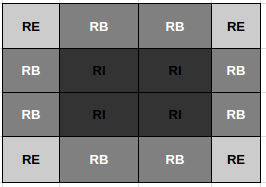
\includegraphics{Chapter2/Chapter2Figs/AHE-interpolacion.png}
    \caption{Interpolación AHE.}
    \label{AHE_Interpolacion}
  \end{center}
\end{figure}

Teniendo en cuenta lo anteriormente descrito, la interpolación de cada píxel en la imagen considera uno de los siguientes casos: 
\begin{itemize}
 \item Si el píxel pertenece a la región interna (RI), entonces interpolar usando las cuatro funciones de transformación adyacentes (arriba izquierda, arriba derecha, abajo izquierda y abajo derecha).
 \item Si el píxel pertenece a una región del borde (RB), entonces interpolar usando las dos funciones de transformación adyacentes (izquierda y derecha o arriba y abajo).
 \item Si el píxel pertenece a una región de esquina (RE), entonces interpolar usando la función de transformación que contiene al píxel.
\end{itemize}

El pseudocódigo del algoritmo $AHE$ se presenta en el Algoritmo \ref{pseudocodigo_ahe}.

\begin{algorithm}
    \begin{algorithmic}[1]
    \REQUIRE $Imagen$ $Original$, Región contextual $(\mathcal{R}_i,\mathcal{R}_j)$: : Se recibe como parámetros la imagen original y la región contextual con dimensiones definidas en $(\mathcal{R}_i,\mathcal{R}_j)$.
    \STATE Dividir $Imagen$ $Original$ en regiones contextuales de tamaño $(\mathcal{R}_i,\mathcal{R}_j)$
    \FOR {Cada Región Contextual}
    \STATE Realizar la Ecualización del Histograma utilizando los pixeles contenidos en la Región Contextual.
    \ENDFOR
    \FOR {Cada Región Contextual}
    \STATE Realizar la interpolación en los pixeles de los bordes para evitar inconsistencias.    \ENDFOR
    \RETURN $Imagen$ $Resultado$: Cuando termine el ciclo iterativo, se retorna una Imagen resultado.
    \end{algorithmic}
    \caption{Pseudocódigo del algoritmo de $AHE$.}
    \label{pseudocodigo_ahe}
\end{algorithm} 

Un problema asociado al proceso $AHE$ es la amplificación del ruido en regiones homogéneas, debido a que la función de transformación satura rápidamente los valores de intensidad \cite{Zuiderveld1994}. En la Figura \ref{cameramanAHE} se muestra un ejemplo de una imagen mejorada utilizando la técnica $AHE$.

\begin{figure}[H]
  \begin{center}
   \captionsetup[figure]{labelformat=empty}
        \subfigure[][]{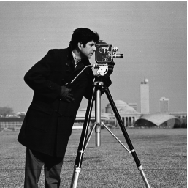
\includegraphics[width=5cm]{cameramanAHE_orig.png}}
        \subfigure[][]{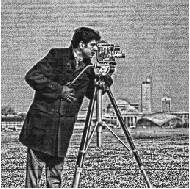
\includegraphics[width=5cm]{cameramanAHE_mej.png}}
    \caption{(a) Imagen Original. (b) Imagen mejorada utilizando AHE.}
    \label{cameramanAHE}
  \end{center}
\end{figure}


\section{Contrast Limited Adaptive Histogram Equalization (CLAHE)}

$CLAHE$ \cite{Zuiderveld1994} se basa en la ecualización adaptativa del histograma $AHE$, donde el histograma se calcula para la región contextual de un píxel.

$CLAHE$ divide a la imagen en regiones y aplica ecualización de histograma a cada una de las regiones, modificando la intensidad de los valores de la imagen mediante una metodología no lineal maximizando el valor de todos los pixeles de la imagen. Fue diseñado pensando en imágenes médicas y ha demostrado ser satisfactorio para mejorar imágenes de bajo contraste \cite{SMG11,MR13}.

$CLAHE$ es un refinamiento de $AHE$ donde el cálculo de realce se modifica agregando un límite para la mejora de contraste, con un parámetro llamado Clip Limit $\mathscr{C}$, este parámetro limita la cantidad de pixeles que puede alcanzar un determinado nivel de gris. La mejora se reduce de este modo en zonas muy uniformes de la imagen, lo que evita un aumento excesivo del ruido y resuelve el problema de “sobre mejora de contraste” del $AHE$.

En las regiones donde existen niveles de gris homogéneos en la imagen se genera un pico sobresaliente en el histograma, $CLAHE$ recorta una parte del pico y redistribuye uniformemente los valores recortados sobre todo el histograma de la región contextual como se ve en la Figura \ref{clahe_recorte_pico}, para mantener el número total de pixeles en la imagen. A partir del histograma recortado se genera la función de transformación \cite{Zuiderveld1994,byong2013}.

\begin{figure}[H]
  \begin{center}
    \leavevmode
    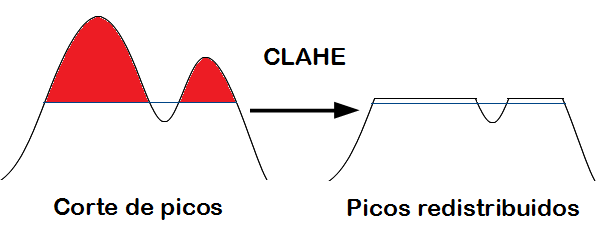
\includegraphics[width=12cm] {distribucion_pixel_clahe.png}
    \caption{Redistribución de pixeles a lo largo del histograma de la región contextual.}
    \label{clahe_recorte_pico}
  \end{center}
\end{figure}

El tamaño de la región contextual de los pixeles y el nivel de Clip Limit $\mathscr{C}$ del histograma son los parámetros de $CLAHE$. Si se define un $\mathscr{C}$ bajo, la pendiente en los histogramas locales generados será también baja, que resultará en poca mejora de contraste. Si se define un $\mathscr{C}$ alto, estaríamos evitando la redistribución de los pixeles que aparecen en los picos del Histograma, lo que resulta ser equivalente a la mejora del $AHE$.

El pseudocódigo del algoritmo $CLAHE$ se presenta en el Algoritmo \ref{pseudocodigo_clahe}.

\begin{algorithm}
    \begin{algorithmic} [1]
    \REQUIRE $Imagen$ $Original$, Región contextual $(\mathcal{R}_i,\mathcal{R}_j)$, Clip Limit $\mathscr{C}$: Se recibe como parámetros la imagen original y la región contextual con dimensiones definidas en $(\mathcal{R}_i,\mathcal{R}_j)$ y el nivel de Clip Limit $\mathscr{C}$.
    \STATE Dividir $Imagen$ $Original$ en regiones contextuales de tamaño $(\mathcal{R}_i, \mathcal{R}_j) $
    \FOR {Cada Región Contextual}
    \STATE Realizar la Ecualización del Histograma utilizando los pixeles contenidos en la Región Contextual.
    \STATE Realizar el Recorte del Histograma de acuerdo con el límite establecido (Clip Limit $\mathscr{C}$)
    \ENDFOR
    \FOR {Cada Región Contextual}
    \STATE Realizar interpolación en los pixeles de los bordes para evitar inconsistencias
    \ENDFOR
    \RETURN $Imagen$ $Resultado$: Cuando termine el ciclo iterativo, se retorna una Imagen resultado.
    \end{algorithmic}
    \caption{Pseudocódigo del $CLAHE$.}
    \label{pseudocodigo_clahe}
\end{algorithm}\break

Las ventajas principales del algoritmo $CLAHE$ son:
\begin{itemize}
    \item Sus requisitos computacionales son relativamente modestos \cite{Zuiderveld1994}.
    \item Es de fácil aplicación, debido a que solamente se deben emplear como parámetros: la región contextual $(\mathcal{R}_i, \mathcal{R}_j)$, y el coeficiente Clip Limit $(\mathscr{C})$ \cite{Zuiderveld1994}.
    \item Provee resultados satisfactorios en imágenes médicas y de bajo contraste \cite{SMG11}.
\end{itemize}

Sin embargo, $CLAHE$ requiere de una minuciosa selección de los valores del tamaño de región contextual $\mathcal{R}$ y el Clip Limit $\mathscr{C}$. Una mala selección de valores podría resultar en amplificación del ruido en la imagen, lo que degrada la calidad de visualización de esta \cite{pisano1998}. Una mala selección del Clip Limit $\mathscr{C}$ puede hacer que no exista corte de picos, lo que puede dar como resultado una mejora equivalente a la del $AHE$.

Para que el resultado de $CLAHE$ sea satisfactorio, los valores de sus parámetros deben ser los óptimos, pero el espacio de búsqueda de los valores para los parámetros es muy grande. Por ello, para encontrar los valores óptimos se necesita un mecanismo que explore el espacio de búsqueda hasta encontrar la solución.

En la Figura \ref{clahe_ahe} se ve un ejemplo de una imagen mejorada con la técnica $AHE$ y con la técnica $CLAHE$. La imagen mejorada con la técnica $CLAHE$, muestra mejor los detalles de esta; y la imagen mejorada con la técnica $AHE$, si bien mejoró la imagen, se observa una zona con mucho brillo.


\begin{figure}[H]
    \captionsetup[figure]{labelformat=empty}
    \centering
        \subfigure[][]{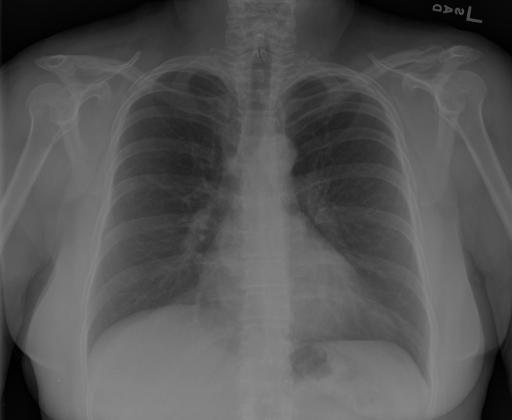
\includegraphics[width=6cm]{imagen12.png}}
        \subfigure[][]{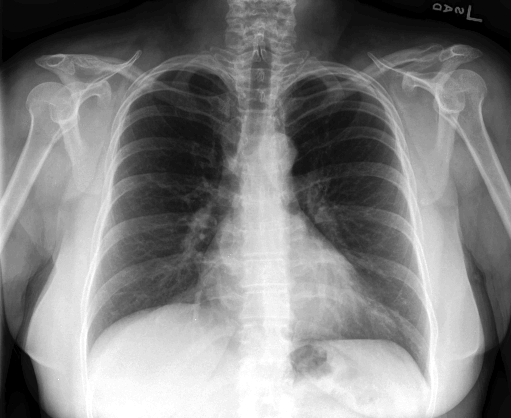
\includegraphics[width=6cm]{imagen12_AHE.png}}
        \subfigure[][]{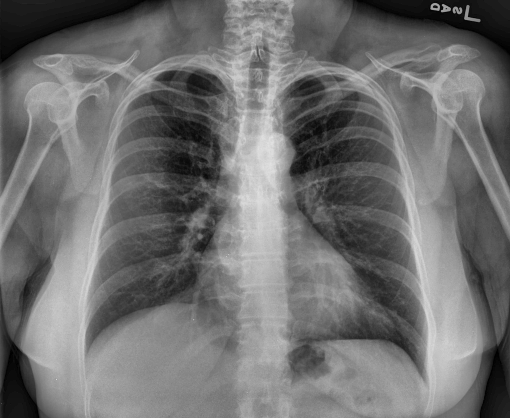
\includegraphics[width=6cm]{imagen12_clahe.png}}
    \caption{(a) Imagen Original. (b) Imagen mejorada con AHE. (c) Imagen mejorada con CLAHE}
    \label{clahe_ahe}
\end{figure}